\documentclass[12pt]{article}
%\documentclass{article}
\usepackage[square,sort,comma,numbers]{natbib}


\usepackage[nottoc, notlot, notlof]{tocbibind}
\renewcommand{\bibname}{Reference}


\usepackage{amsfonts}
\usepackage{mathrsfs}

\usepackage{amsmath}
\usepackage{amsthm}
\usepackage{natbib}
\usepackage{hyperref}
\usepackage{verbatim}
\usepackage{graphicx}


\hypersetup{
	colorlinks,
	citecolor=cyan,
	linkcolor=black,
}

\title{Tensor Decomposition: Algorithms, Error Analysis and Parallelization}
\author{Hao SONG\\{\small Advisor: Laura GRIGORI}}


\begin{document}

\maketitle
\tableofcontents
\newpage

\newtheorem{mydef}{Definition}
\newtheorem{myprop}{Proposition}
\newtheorem{mythm}{Theorem}
\newtheorem{mylem}{Lemma}
\newtheorem{mycor}{Corollary}
\newtheorem{mynot}{Notation}
\newtheorem{myrmk}{Remark}
\newtheorem{myalgo}{Algorithm}
\newtheorem{myprob}{Problem}

\section{Introduction}

Tensor is a multidimensional array, it is a natural generalization of matrix. A matrix $A$ of size $m \times n$ can be regarded as a map
$$ A : \mathbb{R}^m \times \mathbb{R}^n \rightarrow \mathbb{R},$$
while a tensor $\mathcal{A}$ of size $n_1 \times n_2 \times \dots \times n_d$ is a map
$$ \mathcal{A} : \mathbb{R}^{n_1} \times \mathbb{R}^{n_2} \times \dots \times \mathbb{R}^{n_d} \rightarrow \mathbb{R}. $$

In spite of the similarity with respect to their definitions, the actual relationship between matrix and tensor is subtle. The maturity of matrix theory is mostly based on the fact that a matrix is not only a representation of 2 dimensional data, but also a representation of a linear operator. The viewpoint of a linear operator provides matrix with tremendous tools to analyze its decomposition and approximation. Unfortunately, tensor doesn't inherit this advantage. In the domain of tensor decomposition, it can only be interpreted as a collection of data of a multidimensional nature.

The disparity between tensor and matrix theory, to some extent, has triggered more researches exploring multiple aspects of the tensor structure. For instance, 2 earliest tensor decomposition methods, CP decomposition and Tucker decomposition, are generalizations of the matrix singular value decomposition from different perspectives. It turns out that none of these generalizations has all the attractive properties of a matrix singular value decomposition. Instead, CP decomposition has many pathological behaviors, which are indeed one of the major topics of the early research in tensor factorization.

However, although the theoretical part of tensor decomposition is far from mature, its application to realistic practice has already covered a immense domain, including signal analysis, image process, and computational chemistry, etc. \cite{koldaapp} contains a comprehensive introduction to tensor application domains until 2009.

In recent years, with the rapid and steady growth of the computational capability, the types of task that can be tackled by computer and algorithm have been extended to an unprecedented scope. Associated with real world demands, now one of the most prolific domain in computer science is machine learning and data mining. In order to extract meaningful and intrinsic information inside a large collection of data, many techniques in statistic theory specialized to data analysis have to be used. In realistic circumstances, a result is usually related to multiple influence factors, which gives rise to a natural tensor representation. Thus tensor decomposition schemes have considerable applications in this area. In \cite{tensorapprecom}, a recommendation system based on tensor factorization is introduced. \cite{tensorappmining1} \cite{cpnetmining} are examples of complex network analysis using CP and Tucker decomposition. In \cite{tensorappvision}, non-negative tensor decomposition is utilized to the domain of computer vision. Furthermore, in \cite{tensorapplearn1}, a systematical approach is described to employ tensor decomposition in latent variable models, which has applications in natural language processing \cite{tensorapplang}. 

In fact, as a historical note, some of the tensor decomposition schemes are invented for the very purpose of interpreting the intrinsic relations hiding behind multidimensional data. For example, \cite{Tucker1966} is the original paper introducing the Tucker factorization in 1960s, where the main purpose of this factorization was to reveal the influence of multiple factors in psychology.

On the other hand, tensor decomposition without any semantic interpretation can still be useful. Another area where tensor is widely used is data compression, both for data of relatively low dimension and extremely high dimension. In such cases, tensor decomposition is mainly a means to approximate data with drastic reduction of its size, while whether such decomposition is meaningful doesn't matter. For low dimensional data, Tucker approximation has been considered as a data compression technique for a long time. Since the amount of data from scientific computing has become increasingly large, a reasonable approximation with high accuracy is indeed necessary. In \cite{koldapara}, a parallel Tucker decomposition is implemented, demonstrating a huge degree of compression with only a little loss of precision. 


Meanwhile, the compression of a tensor with tremendously high dimension has attracted much intention in the latest advances of tensor based low rank approximation as well. Partly because of the numerical analysis involving stochastic partial PDEs and other PDEs with enormous size of parameters, where a representation of a function with even more than 1000 parameters are demanded, new innovations in tensor approximation have been put forward in the last ten years. In \cite{ttree} and \cite{ttrain}, new tensor decomposition formats, Tensor Tree and Tensor Train format, which are particularly adapted to high dimensional tensors, are introduced. Furthermore, \cite{thiera} proposes a more general scheme utilizing a hierarchical representation. These new formats, to some extents, has become the data structure of multivariate function itself, since many algebraic operation are supported natively without the need to retrieve the original format. For example, \cite{ttrainsolve} presents a way to solve linear system with all terms involved represented as tensors in Tensor Train format. A comprehensive literature survey of latest progresses until 2013 focusing on low rank approximation can be found in \cite{lowranklit}. 

In this report, we will explore some widely used tensor decomposition formats in detail. Special focus will be put on the systematical analysis of existing algorithms, as well as their theoretical error estimation. Error estimation consists of 2 aspects, the \textit{a priori} estimate in term of the relation between an algorithm and the best possible result in theory, and the \textit{a posteriori} estimate calculating the real final error by the known real error introduced in each computing stage. On the way of describing and analyzing these well-known algorithms, some new contributions of the report will be presented, among which are the subsections Randomized Algorithm, QRCP Based Algorithm and Further Generalization in Section 3. At the best of the author's knowledge, these results have not been shown in the literature. Some of the known parallel algorithms will be included briefly, and we will underline some key points of the parallelization of our new algorithms.




\section{CP(CANDECOMP/PARAFAC) Decomposition}

The concept of CP decomposition dates back to 1920s. After several re-introductions, this decomposition format has become one of the most used tensor decompositions these days. We refer to \cite{koldaapp} for a concise historical introduction of CP decomposition. 

Mathematically, CP decomposition is a natural generalization of a particular interpretation of the matrix SVD decomposition. Let $A$ be a matrix of size $m \times n$, When we perform a SVD on $A$, we get
$$ A = U \Sigma V^T, $$
where $U, V$ are orthogonal matrices of size $m \times m$ and $n \times n$ respectively, and $\Sigma$ is a diagonal matrix whose diagonal line consists of all singular values in decreasing order. 

We regard $U$ as a juxtaposition of orthonormal column vectors: $U = (u_1, \dots, u_m)$, where $u_1 \dots u_m$ are vectors of size $m$. Similarly, $V = (v_1, \dots, v_n)$. If $\sigma_1, \dots, \sigma_r $, where $1 \leq r \leq \min(m, n)$ is the rank of $A$, are all the singular values of $A$, then the decomposition above can be simply rewritten as
$$ A = \sum_{i = 1}^r \sigma_i u_i v_i^T.$$

Notice that $u_iv_i^T$ can be considered as a means to to construct a rank-1 matrix of size $m \times n$ from 2 vectors of size $m$ and $n$ respectively, which is a motivation of the following definition:

\begin{mydef}
Let $a^1, \dots a^d$ be $d$ vectors, where $a^i$ is of size $n_i$, $\forall 1 \leq i \leq d$. Then tensor $a^1 \otimes a^2 \dots \otimes a^d$ is defined element-wise by:
$$ (a^1 \otimes a^2 \dots \otimes a^d)(i_1, i_2, \dots, i_d) := a^1(i_1) a^2(i_2) \dots a^d(i_d),$$
where $1 \leq i_s \leq n_s$ for all $1 \leq s \leq d$. Furthermore, we call any tensor of this form a rank-1 tensor.
\end{mydef}

\begin{mydef}{(CP decomposition)}
\label{defcp}
Let $\mathcal{A}$ be a tensor of size $n_1 \times \dots \times n_d$, a CP decomposition of $\mathcal{A}$ with $r$ components is of the form:
$$ \mathcal{A} \approx \sum_{i = 1}^r \lambda_i u_i^1 \otimes u_i^2 \otimes \dots \otimes u_i^d,$$
where $u_i^s$ is a vector of size $n_s$ and Euclidian norm 1, for all $1 \leq s \leq d$, and $1 \leq i \leq r$.
\end{mydef}

CP decomposition has attracted many theoretical studies, despite of its rather pathological behavior comparing with its matrix counterpart. We will illustrate some of the most remarkable properties:

First part is about the exact decomposition of minimal number of components. Traditionally, the rank of a tensor is defined as the smallest $r$ in the definition above, together with those $u_i^s$, $1 \leq s \leq d$, and $1 \leq i \leq r$, such that the decomposition above is an exact equality:
$$ \mathcal{A} = \sum_{i = 1}^r \lambda_i u_i^1 \otimes u_i^2 \otimes \dots \otimes u_i^d.$$

In the case of a matrix, such exact decomposition is provided by SVD algorithm. However, for the general CP decomposition, the problem of determining the tensor rank has been proved to be NP-complete (see \cite{cpnpcomplete}). Hence it is impossible to determine this rank in practice, not to mention an algorithm to compute an instance of this exact CP decomposition.

Moreover, even if we only expect an approximation, the situation is still bizarre, because the notion of best low rank approximation with the number of components fixed can be ill-posed. The phenomenon of ill-posedness is largely due to the cancellation effect. That is, the magnitude of every individual tensor becomes infinitely large, and meanwhile, the final sum tends increasingly close to the original tensor as a result of mutual cancellation. Thus, when using CP decomposition as a tactic of approximation, the concept of best approximation might be totally meaningless. See \cite{cpill} for more details.

\subsection{ALS Algorithm}
Since the theoretical properties of CP decomposition is quite pathological, there are no known algorithms allowing an \textit{a priori} estimate of the approximation error. And nearly all algorithms to compute the CP decomposition are based on optimization.

A widely used algorithm for CP decomposition is the ALS (Alternating Least Square) algorithm. When the number of components $r$ in the definition of CP decomposition is fixed, we can reformulate the CP decomposition as a optimization problem:

\begin{myprob}
For a given tensor $\mathcal{A}$ with size $n_1 \times \dots \times n_d$,
find $u_i^s$, $1 \leq i \leq r$, $1 \leq s \leq d$, such that they minimize: 
 $$|| \mathcal{A} - \sum_{i = 1}^r u_i^1 \otimes u_i^2 \otimes \dots \otimes u_i^d ||.$$
\end{myprob}

Notice that for symmetry, here we let $u_i^1$ absorb the scalar $\lambda_i$ for all $1 \leq i \leq r$, thus the expression looks slightly different to the one used in Definition \ref{defcp}.

We denote 
$$U_s := (u_1^s, \dots, u_r^s)$$ 
as a matrix of size $n_s \times r$ for all $1 \leq s \leq d$. An observation is, when $U_2, \dots, U_d$ are fixed, the optimization problem above with respect to $U_1$ is linear. Thus it can be solved by the standard least square method. What the ALS algorithm does is to solve these least square problems successively for $U_1, U_2, \dots$ until $U_d$. And then repeat the whole process. Continue until some stopping conditions are satisfied.

\begin{myalgo}{(ALS for CP decomposition)}
We keep the notation in this subsection, then the algorithm is as follows:
\begin{itemize}
\item initialization: guess an initial value for each $U_1, \dots, U_d$
\item label: 
	\begin{itemize}
		\item for i from 1 to d: \\
			fix $U_j, \forall 1 \leq j \leq d \text{ and } j \neq i$, solve the optimization problem for $U_i$ by least square method, and update $U_i$ to the minimizer.
		\item check for stopping condition (possibly, the stopping condition can be 1, the decreasing of objective function is stagnant; 2, the objective function is small enough; 3, maximum iteration number reached; etc.), 
			if stopping condition is not satisfied, go to "label".
	\end{itemize}
\item finalization: output $U_1, \dots, U_d$
\end{itemize}
\end{myalgo}

Since the objective function is reduced after every step of least square method, the ALS algorithm will converge to some point theoretically. However, there is no guarantee that this final convergence point is a global or even local minimizer. And the speed of convergence can be very slow. Both the quality of the result and the speed of convergence depend on the initial guess.

Considering the usefulness of CP decomposition in a wide range of application domains, there are many parallel algorithms for CP decomposition and its variants. For instance, in \cite{cpgigatensor}, a parallel implementation of CP decomposition is presented, which employs MapReduce, a famous distributed computing framework in the last decade. 

\section{Tucker Decomposition}
For the sake of simplicity, we fix a tensor $\mathcal{A}$ of size $n_1 \times n_2 \times \dots \times n_d$ in this section. And as a well accepted convention, in the context of tensor decomposition, the index $i$ is called the mode $i$.

Tucker decomposition is based on the observation that a tensor can be naturally regarded as a collection of vectors. For any fix $1 \leq k \leq d$, we let the mode $k$ to be special, and consider the set $Vec_k(\mathcal{A})$ comprised of all vectors for a fix tuple of values of other modes:
$$
Vec_k(\mathcal{A}) := \{ 
\begin{pmatrix}
\mathcal{A}(i_1, ..., 1, ..., i_d) \\
\mathcal{A}(i_1, ..., 2, ..., i_d) \\
\vdots   \\
\mathcal{A}(i_1, ..., n_k, ..., i_d)
\end{pmatrix}
: 1 \leq i_s \leq n_s, \forall 1 \leq s \leq d, s \neq k\}
$$
Thus $Vec_k(\mathcal{A})$ is a subset of $\mathbb{R}^{n_k}$ with $\Pi_{i \neq k}n_i$ elements, which allows us to perform matrix multiplication simultaneously to all these vectors yielding another vector collection of different but uniform size. Moreover, the resulting collection of vectors can be considered as a tensor in a natural way, resembling the recovery from $Vec_k(\mathcal{A})$ to $\mathcal{A}$ itself.

A particular emphasis should be made here for the importance of alternating among different viewpoints to look at a tensor. When one mode is specialized, we get a collection of vectors; once these vectors are put together consecutively in a specific order, a matrix is produced. If furthermore, the order of placement is standardized, then this matrix records all the information to be recovered back to the original tensor. For Tucker decomposition, a naive approach stated here is enough to introduce all the essential parts. Nevertheless, for more complicated decomposition scheme like Tensor Train decomposition, we need more general notions to articulate the multiple ways of transformation between a tensor and a matrix, which will be defined in later sections.

The following is a formal definition of tensor matrix multiplication:

\begin{mydef}{(Tensor Matrix Multiplication)}
Let $\mathcal{A}$ be a tensor of size $n_1 \times n_2 \times \dots \times n_d$, $M$ be a matrix of size $m \times n_k$ where $1 \leq k \leq d$. Then the tensor matrix production $\mathcal{A} \times_k M$ is a tensor of size $n_1 \times \dots n_{k-1} \times m \times n_{k+1} \times \dots \times n_d$ defined element-wise by:
\begin{alignat*}{9}
& (\mathcal{A} \times_k M)(i_1, \dots, i_{k-1}, s, i_{k+1}, \dots, i_d) \\
:= &\sum_{t = 1}^{n_k} M(s, t) A(i_1, \dots, i_{k-1}, t, i_{k+1}, \dots, i_d),
\end{alignat*}
for $1 \leq s \leq m$ and $1 \leq i_l \leq n_l, \forall 1 \leq l \leq d, l \neq k$
\end{mydef}

\begin{mynot}
The notation $\times_k$ will be interpreted as left associative. To be precise, $\mathcal{A} \times_{k_1} M_1 \times_{k_2} M_2 := (\mathcal{A} \times_{k_1} M_1) \times_{k_2} M_2 $. We can easily deduce that the order of multiplication doesn't matter as long as $k_1 \neq k_2$.
 \end{mynot}

\begin{myprop}{(Commutativity)}
Let $1 \leq k_1 < k_2 \leq d$, $M_1$ of size $m_1 \times n_{k_1}$, $M_2$ of size $m_2 \times n_{k_2}$, then 
$$\mathcal{A} \times_{k_1} M_1 \times_{k_2} M_2 = \mathcal{A} \times_{k_2} M_2 \times_{k_1} M_1$$
\end{myprop}
\begin{proof}
\begin{alignat*}{9}
& (\mathcal{A} \times_{k_1} M_1 \times_{k_2} M_2)(\dots, s_1, \dots, s_2, \dots) \\
= & \sum_{j = 1}^{n_{k_2}} M_2(s_2, j) (\mathcal{A} \times_{k_1} M_1)(\dots, s_1, \dots, j, \dots) \\
= & \sum_{j = 1}^{n_{k_2}} M_2(s_2, j) ( \sum_{i = 1}^{n_{k_1}} M_1(s_1, i) A(\dots, i, \dots, j, \dots) ) \\
= & \sum_{i = 1}^{n_{k_1}} \sum_{j = 1}^{n_{k_2}} M_1(s_1, i) M_2(s_2, j) A(\dots, i, \dots, j, \dots) .
\end{alignat*}
Therefore, by symmetry, 
\begin{alignat*}{9}
&( \mathcal{A} \times_{k_2} M_2 \times_{k_1} M_1 ) ( \dots, s_1, \dots, s_2, \dots ) \\
= & \sum_{i = 1}^{n_{k_1}} \sum_{j = 1}^{n_{k_2}} M_1(s_1, i) M_2(s_2, j) A(\dots, i, \dots, j, \dots),
\end{alignat*}
which leads to the equality in the proposition.
\end{proof}

Now we have all the prerequisites to introduce the Tucker decomposition. Intuitively speaking, Tucker decomposition is processed by applying a tensor matrix multiplication on every mode to reduce the size of the remaining tensor. For example, multiplying a matrix of size $m \times n_k$ to a tensor of size $n_1 \times \dots \times n_d$ yields a tensor of size $n_1 \times \dots \times n_{k-1} \times m \times n_{k+1} \times \dots \times n_d$. In this procedure, we eliminate $(n_k - m)\Pi_{i \neq k} n_i$ elements at the cost of introducing $m \times n_k$ new elements. Normally, the former is much bigger than the latter, leading an effective way of compression. A formal definition is as follows:

\begin{mydef}{(Tucker Decomposition)}
\label{tuckerd}
Let $\mathcal{A}$ be a tensor of size $n_1 \times \dots \times n_d$. $U_i, 1 \leq i \leq d$ be a collection of matrices of size $n_i \times m_i$ respectively, such that for every $U_i$, $1 \leq i \leq d$, all its columns are orthonormal. Then a Tucker decomposition with respect to these orthogonal matrices is a core tensor $\mathcal{B}$:
$$ \mathcal{B} := \mathcal{A} \times_1 U_1^T \times_2 \dots \times_d U_d^T.$$
As a means of approximation, one can retrieve an approximative matrix $\tilde{\mathcal{A}}$ of $A$ by
$$ \tilde{\mathcal{A}} :=  \mathcal{B} \times_1 U_1 \times_2 \dots \times_d U_d.$$. 
\end{mydef}


From the commutativity above, $\tilde{\mathcal{A}}$ is actually:
$$ \tilde{\mathcal{A}} = \mathcal{A} \times_1 U_1 U_1^T \times_2 \dots \times_d U_dU_d^T.$$
Notice that the matrices $U_iU_i^T$, $1 \leq i \leq d$ are orthogonal projections, we can exploit this property to obtain some general error bounds.

\begin{mydef}{(Frobenius Norm)}
Let $\mathcal{A}$ be a tensor of size $n_1 \times \dots \times n_d$, its Frobenius norm $|| \mathcal{A}||$ is defined by
$$|| \mathcal{A}|| := \sqrt{ \sum_{i_1, i_2, \dots, i_d} |A(i_1, i_2, \dots, i_d)| ^ 2 }$$
\end{mydef}

We mention here that all tensor norms $|| \cdot || $ used in the sequel refer to this Frobenius norm. And all matrix norms used afterwards are matrix Frobenius norm.

\begin{myprop}
Let $\mathcal{A}$ be a tensor of size $n_1 \times \dots \times n_d$, and $M$ be a matrix of size $m \times n_k$ with some $1 \leq k \leq d$ whose columns are orthonormal. Then 
$$ || \mathcal{A} \times_k M || \leq || \mathcal{A} || $$
\end{myprop}

\begin{proof}
It is evident from the fact that such matrix reduces the $l_2$ norm of every column.
\end{proof}

The following theorem provides a precise formula to compute the final error accumulated by each step:
\begin{mythm}
\label{tuckerm1}
Let $\mathcal{A}$ be a tensor of size $n_1 \times \dots \times n_d$. Fix $1 \leq s \leq d$ and a collection of distinct numbers $\{p_1, \dots, p_s\} \subseteq \{1, \dots, d\}$. Let $\pi_{p_i}$, $1 \leq i \leq s$ be orthogonal projections of size $n_{p_i} \times n_{p_i}$ respectively.
Then 
\begin{alignat*}{9}
& || \mathcal{A} - \mathcal{A} \times_{p_1} \pi_{p_1} \dots \times{p_s} \times_{p_s} \pi_{p_s}||^2 \\
= & || \mathcal{A} - \mathcal{A} \times_{p_1} \pi_{p_1} ||^2 + || \mathcal{A} \times_{p_1} \pi_{p_1} - \mathcal{A} \times_{p_1} \pi_{p_1} \times_{p_2} \pi_{p_2} || ^ 2 +  \\
& \dots + || \mathcal{A} \times_{p_1} \dots \times_{p_{s-1}} \pi_{p_{s-1}} - \mathcal{A} \times_{p_1} \dots \times_{p_{s-1}} \pi_{p_{s-1}} \times_{p_s} \pi_{p_s} || ^2
\end{alignat*}
\end{mythm}

\begin{proof}
\begin{alignat*}{9}
& || \mathcal{A} - \mathcal{A} \times_{p_1} \pi_{p_1} \dots \times{p_s} \times_{p_s} \pi_{p_s}||^2 \\
= & || (\mathcal{A} - \mathcal{A} \times_{p_1} \pi_{p_1}) + (\mathcal{A} \times_{p_1} \pi_{p_1} - \mathcal{A} \times_{p_1} \pi_{p_1} \dots \times{p_s} \times_{p_s} \pi_{p_s} || ^2 \\
= & || \mathcal{A} \times_{p_1} (I - \pi_{p_1}) + (\mathcal{A} - \mathcal{A} \times_{p_2} \dots \times_{p_s} \pi_{p_s}) \times_{p_1} \pi_{p_1} || ^2 \\
= & || \mathcal{A} \times_{p_1} (I - \pi_{p_1})|| ^2 + ||(\mathcal{A} - \mathcal{A} \times_{p_2} \dots \times{p_s} \pi_{p_s}) \times_{p_1} \pi_{p_1} || ^2 \\
= & || \mathcal{A} - \mathcal{A} \times_{p_1} \pi_{p_1} ||^2 + || (\mathcal{A} \times_{p_1} \pi_{p_1}) - (\mathcal{A} \times_{p_1} \pi_{p_1}) \times_{p_2} \dots \times_{p_s} \pi_{p_s} || ^ 2
\end{alignat*}
Notice that the second term can be expanded recursively, thus the original identity is proved.
\end{proof}

Now we need to introduce the concept of the best approximation with a fixed core tensor size, which would be useful as a reference frame to examine the theoretical accuracy of the results produced by various algorithms. As we have mentioned before, for CP decomposition, the problem of best low rank approximation is ill-posed. Fortunately, for the approximation in Tucker format, a best approximation is well-defined.

\begin{myprop}{(Existence of the Best Approximation)}
Let $\mathcal{A}$ be a tensor of size $n_1 \times \dots \times n_d$. Fix a tuple of numbers $(m_1, \dots, m_d)$ that satisfies $1 \leq m_i \leq n_i$, $\forall 1 \leq i \leq d$. Let $\mathscr{S}$ be the collection be all possible approximations of $\mathcal{A}$ for core tensor size  $(m_1, \dots, m_d)$, that is:
\begin{alignat*}{9}
\mathscr{S} := \{ \mathcal{B} \times_1 M_1 \dots \times_d  M_d: \mathcal{B} \text{ is a tensor of size } (m_1, \dots, m_d),  \\
M_i \text{ is a matrix of size } n_i \times m_i, \forall 1 \leq i \leq d \},
\end{alignat*}
Then there exists $\mathcal{A}_{best} \in \mathscr{S}$, such that
$$ || \mathcal{A} - \mathcal{A}_{best} || \leq || \mathcal{A} - \mathcal{C} || \text{, for all } \mathcal{C} \in \mathscr{S} $$
\end{myprop}

\begin{proof}
This is almost a direct corollary of the existence of the minimal value for a continuous function defined in a compact space.
\end{proof}

\begin{myrmk}
In the previous proposition, we haven't imposed the restriction that $M_i$, $1 \leq i \leq d$ should have orthonormal columns. Actually, it doesn't matter. Since otherwise, we can perform an economic QR factorization on $M_i$, and let the core tensor absorb the $R$ part, which implies that the collection $\mathscr{S}$ remains the same if we add the orthogonality restriction on $M_i$.

\end{myrmk}


For the subsequent part, we fix some notations for simplicity:
\begin{mynot}
We use $\sigma_i(A)$ to denote the $i$th biggest singular value for any matrix $A$ without explicit declaration.
\end{mynot}

\subsection{HOSVD Algorithm}

The most natural way to obtain a Tucker decomposition is by applying truncated SVD algorithm to each mode of the tensor. This is called an HOSVD (High Order Singular Value Decomposition) algorithm. However, one might imagine 2 slightly different approaches.

\paragraph{Traditional HOSVD algorithm} For $\forall 1 \leq i \leq d$, juxtapose all vectors in $Vec_i$ to form a matrix. Then compute a truncated SVD decomposition for this matrix to obtain a set of orthonormal columns as a matrix $U_i$ of size $n_i \times m_i$. Finally, since all $U_i$, $1 \leq i \leq d$ have been computed, we can assemble the core tensor $\mathcal{B}$ simply by 
$$ \mathcal{B} := \mathcal{A} \times_1 U_1^T \times_2 \dots \times_d U_d^T.$$

This is the traditional way to compute HOSVD. We can analyze the error produced by this approach by utilizing the theorem above, leading the corollary as follows:

\begin{mycor}
Let $\mathcal{B}$ be the core tensor computed by the Traditional HOSVD algorithm, and $\tilde{\mathcal{A}} := \mathcal{B} \times_1 U_1 \times_2 \dots \times_d U_d$ be the approximate tensor recovered from this core tensor. Then the error between $\tilde{\mathcal{A}}$ and the original one is bounded by:
$$|| \mathcal{A} - \tilde{\mathcal{A}} || ^ 2 \leq \sum_{i = 1}^d || \mathcal{A} - \mathcal{A} \times_{p_i} U_{p_i} U_{p_i}^T||^2. $$
Moreover, if we denote $\mathcal{A}_{best}$ to be the best approximation for the same fixed core tensor size, then $\tilde{\mathcal{A}}$ computed above satisfies:
$$ || \mathcal{A} - \tilde{\mathcal{A}} || \leq \sqrt{d} || \mathcal{A} - \mathcal{A}_{best}||$$
\end{mycor}

\begin{proof}
We have proved that an orthogonal matrix will never increase the norm of a tensor. Thus the theorem above becomes
$$|| \mathcal{A} - \mathcal{A} \times_{p_1} \pi_{p_1} \dots \times{p_s} \times_{p_s} \pi_{p_s}||^2 \leq \sum_{i = 1}^s || \mathcal{A} - \mathcal{A} \times_{p_i} \pi_{p_i}||^2.$$
Therefore, if we set $s = d$ and $p_i = i$ for all $1 \leq i \leq d$, we obtain the first inequality directly.

For the second part, we recall that the truncated SVD algorithm provides the best approximation for a fixed rank. Thus
$$ || \mathcal{A} - \mathcal{A} \times_{p_i} U_{p_i} U_{p_i}^T|| \leq || \mathcal{A} - \mathcal{A}_{best} ||, $$
or, $$|| \mathcal{A} - \tilde{\mathcal{A}} || ^ 2 \leq d || \mathcal{A} - \mathcal{A}_{best} || ^2$$
\end{proof}

\paragraph{Sequentially Truncated HOSVD algorithm}
A sequentially truncated HOSVD, by contrast, will not compute the SVD for a fixed tensor $\mathcal{A}$. Instead, after every truncation, the original tensor $\mathcal{A}$ will be updated to reflect this truncation. As the computation processes, the tensor size gets smaller significantly.

\begin{myalgo}
Given a tensor $\mathcal{A}$ of size $n_1 \times \dots \times n_d$ to be factorized. The algorithm for sequentially truncated HOSVD produces a core tensor $\mathcal{B}$ and a collection of matrices $\{U_i\}_{i = 1}^d$ with orthonormal columns: 
\begin{itemize}
\item initialization: set $\mathcal{A}_0 \leftarrow \mathcal{A}$
\item for $i$ from $1$ to $d$: 
	\begin{itemize}
		\item compute $\mathcal{A}_{i-1} \approx \mathcal{A}_i \times_i U_i $ by applying truncated SVD to the matrix formed by all columns in $Vec_{i}(\mathcal{A}_{i-1})$
	\end{itemize}
\item finalization: set $\mathcal{B} \leftarrow \mathcal{A}_d$, obtain $\mathcal{A} \approx  \mathcal{B} \times_1 U_1 \dots \times_d U_d $
\end{itemize}
\end{myalgo}

The previous theorem can be used here without any modification:
\begin{mycor}
\label{hosvdcor}
In the sequentially truncated HOSVD algorithm above, suppose in step $i$, $1 \leq i \leq d$, we introduce an truncation $\epsilon_i$  error in the SVD decomposition, i.e.
$$ \epsilon_i :=  || \mathcal{A}_{i - 1} - \mathcal{A}_i \times_i U_i || $$ 
Then the final approximate $\tilde{\mathcal{A}} :=  \mathcal{B} \times_1 U_1 \dots \times_d U_d $ satisfies:
$$ || \mathcal{A} - \tilde{\mathcal{A}} || ^2  = \sum_{i = 1}^d \epsilon_i^2,$$
Moreover, if $\mathcal{A}_{best}$ is the best approximation in the constraint of the same core tensor size, then 
$$ || \mathcal{A} - \tilde{\mathcal{A}} || \leq \sqrt{d} || \mathcal{A} - \mathcal{A}_{best}||$$
\end{mycor}

\begin{proof}
By the definition of truncated SVD, we have $\mathcal{A}_i = \mathcal{A}_{i-1} \times U_i^T$. Recursively, we get
$$ \mathcal{A}_i = \mathcal{A} \times_1 U_1^T  \dots \times_i U_i^T $$
We have shown that multiplication by $U_i$, a matrix with orthonormal columns, will not change the tensor norm. Therefore
\begin{alignat*}{9}
\epsilon_i & = || \mathcal{A}_{i - 1} - \mathcal{A}_i \times_i U_i || \\
&= || \mathcal{A}_{i-1} \times_1 \dots \times_{i-1} U_{i-1} - \mathcal{A}_i \times_1 \dots \times_i U_i || \\
&= || \mathcal{A} \times_1 \dots \times_{i-1} U_{i-1}U_{i-1}^T - \mathcal{A} \times_1 \dots \times_i U_iU_i^T ||.
\end{alignat*}
On the other hand, $\tilde{\mathcal{A}}$ is actually
\begin{alignat*}{9}
 \tilde{\mathcal{A}} &=  \mathcal{B} \times_1 U_1 \dots \times_d U_d \\
& = \mathcal{A}_d \times_1 U_1 \dots \times_d U_d \\
& = \mathcal{A} \times_1 U_1U_1^T \dots \times_d U_dU_d^T
 \end{alignat*}
By setting $s = d$, $p_i = i, \pi_{p_i} = U_iU_i^T$, $\forall 1 \leq i \leq d$ in the previous theorem, the first part of the conclusion in this corollary is direct.

For the second part, we let $\mathcal{A}_{best,i} := \mathcal{A}_{best} \times_1 \dots \times_{i-1} U_{i-1}^T$. Then 
\begin{alignat*}{9}
& || \mathcal{A} - \mathcal{A}_{best} || \\
 \geq & || \mathcal{A} \times_1 \dots \times_{i-1} U_{i-1}U_{i-1}^T - \mathcal{A}_{best} \times_1 \dots \times_{i-1} U_{i-1}U_{i-1}^T || \\
 \geq & || \mathcal{A}_{i-1} \times_1 \dots \times_{i-1} U_{i-1} - \mathcal{A}_{best, i} \times_1 \dots \times_{i-1} U_{i-1} || \\
 \geq & || \mathcal{A}_{i-1} - \mathcal{A}_{best,i} || \\
 \geq & || \mathcal{A}_{i-1} - \mathcal{A}_{i} \times_i U_i || = \epsilon_i,
\end{alignat*}
and the result becomes apparent.
\end{proof}

The advantage of the sequentially truncated version is multifold. First is the computational cost. Generally, a truncation will perform drastic reduction of the length of a mode being processed. As a consequence, after every step, the computational task for the next step will be largely reduced. Second is the temporary memory use. For the traditional HOSVD, the memory consumption is at a same high level during the whole process. However, for HOSVD with sequential truncation, the memory consumption is high at the beginning, and will decrease gradually as more modes are being computed. 

Final and maybe the most important point is that, statistically, the latter will produce more accurate approximation. Intuitively, the successive removing of irrelevant elements makes the temporary core tensor more concentrated, leading a better accuracy. Although this conclusion is not based on rigorous theoretical proof, and indeed there are counterexamples, for most of the experimental cases, the sequentially truncated HOSVD is much better. 

On the other hand, the HOSVD with sequential truncation has some additional flexibility. In the previous theorem where we deduce an identity for error estimate, the order to process each mode doesn't need to be fixed. In fact, the tuple $(p_1, \dots, p_d)$ can be any permutation of $(1, \dots, d)$. (Note that for the conciseness of the presentation, in the algorithm above, we haven't shown the potential existence of this permutation.) Intuitively, different choices of permutation will lead to different data storage and computational cost in the middle of all steps. It has be shown by experiments. There are also some heuristic approaches to select a better permutation. We refer to \cite{trunctucker} for more details.

A parallel implementation of HOSVD algorithm using multidimensional memory layout can be found in \cite{koldapara}. The key point is how to compute the SVD of a matrix $A$ of size
$n_i \times (n_1 \dots n_{i-1} n_{i+1} \dots n_d)$, which has a remarkable property that the length of a column is much smaller than the length of a row. The parallel implementation in that paper exploits this characteristic, by using $AA^T$ to compute the SVD of $A$. Although this approach might affect the numerical stability, it drastically reduces the computational cost, since the only stage involving communication among different processors is the tensor matrix multiplication.

\subsection{Randomized Algorithm}
We recall the definition of Tucker decomposition, the essential part is some orthogonal columns extracted from every tensor mode, constructing orthogonal projections to approximate the original tensor. HOSVD provides a reliable method to compute these orthogonal columns. However, SVD is not the only algorithm to achieve this goal. In fact, any matrix decomposition of the form 
$$ A \approx QB$$
where $Q$ is an matrix with orthonormal columns and $B$ is computed from $B = Q^TA$, could be a candidate. 

Generally, a matrix with orthonormal columns arises from subspace orthogonal projection, and the QR decomposition is the most usual way to extract such orthogonal vectors from a general matrix. We will explore more on this QR approach later. In this subsection, we will present the use of randomized subspace projection to Tucker decomposition.

In recent years, randomized algorithms have attracted increasingly attention from the scientific computing community, because of the relatively lower computational cost and the robustness. As opposed to the situation decades ago, when the probabilistic approach was immature and unstable, many randomized algorithms these days have solid theoretical guarantee of correctness and time-proven robustness in practice. Some of the the randomized algorithms for matrix at the beginning have already been adapted to Tucker tensor decomposition, see \cite{trand2007} and \cite{trandMACH} for example. What we are interested in is the matrix approximation method proposed in \cite{randAppro} based on random projection.

\begin{myalgo}{(Algoritm 4.1 in \cite{randAppro})}
Given an $m \times n$ matrix $A$, and an integer $l$, the following algorithm computes the an $m \times l$ orthonormal matrix $Q$ whose range space approximates the range space of $A$.
\begin{itemize}
\item Draw an $n \times l$ Gaussian random matrix $\Omega$
\item Construct approximate range space $Y := A\Omega$
\item Orthogonalize $Y$ by QR factorization $Y = QR$
\end{itemize}
\end{myalgo}

We emphasize that we always use the Frobenius norm for both matrix and tensor. In terms of Frobenius error, the random projection above has surprisingly accurate output.

\begin{mythm}{(Theorem 10.7 in \cite{randAppro})}
\label{thmrandappro}
Suppose that $A$ is a $m \times n$ matrix. Choose a target rank $k \geq 2$ and an oversampling parameter $p \geq 2$, with $k + p \leq \min\{m, n\}$. Draw an $n \times (k + p)$ standard Gaussian matrix $\Omega$, and construct the sample matrix $Y = A\Omega$. Let $Q$ denote the orthogonal factor of the QR factorization of  $Y$, i.e. $Y = QR$ for some upper triangular matrix $R$. Then for all $u, t \geq 1$, 
$$ || A - QQ^TA || \leq ( 1 + t \cdot \sqrt{12k/p}) (\sum_{j > k} \sigma_j(A)^2)^{1/2} + ut \cdot \frac{e \sqrt{k+p}}{p+1} \cdot \sigma_{k+1}(A),$$
with failure probability at most $5 t^{-p} + 2 e ^{-u^2 / 2}$.
\end{mythm}

Note that $(\sum_{j > k} \sigma_j(A)^2)^{1/2}$ is indeed the best rank $k$ approximation produced by the truncated SVD. Thus this theorem provides a theoretical bound of the error incurred by the subspace projection algorithm, in terms of the best approximation error we could ever get.
\begin{myrmk}
\label{randBound}
With properly chosen parameters $p, u$ and $t$, this theorem asserts a fairly good error bound. For example, we let $t = u = 4$ and $p = 6$. Then
$$ || A - QQ^TA|| \leq 32 || A - A_{rank\_k_svd} || $$
will hold with failure probability at most $0.0019$.
\end{myrmk}

By applying the subspace projection algorithm to the Tucker decomposition, we have the following randomized Tucker decomposition algorithm:

\begin{myalgo}
Given tensor $\mathcal{A}$ of size $n_1 \times \dots \times n_d$, this algorithm computes a collection of matrices $\{Q_i\}_{i = 1}^d$ with orthonormal columns and a core tensor $\mathcal{B}$. $Q_i$ is of size $n_i \times (m_i + 6)$, $\forall 1 \leq i \leq d$, and $\mathcal{B}$ is of size $(m_1 + 6)  \times \dots \times (m_d + 6)$.
\begin{itemize}
\item initialization: set $\mathcal{A}_0 \leftarrow \mathcal{A}$
\item for i from $1$ to $d$:
	\begin{itemize}
		\item juxtapose columns in $Vec_i(\mathcal{A}_{i-1})$ to form a matrix $C_i$ of size $n_i \times (m_1+6) \dots (m_{i-1}+6)  n_{i+1} \dots n_d $
		\item draw an $(m_1+6) \dots (m_{i-1}+6)  n_{i+1} \dots n_d \times (m_i + 6)$ standard Gaussian matrix $\Omega_i$
		\item compute $Y_i := C_i \Omega_i$, $Y_i$ is of size $n_i \times (m_i + 6)$
		\item compute the QR factorization of $Y_i$: $Y_i = Q_i R_i$
		\item set $\mathcal{A}_i \leftarrow \mathcal{A}_{i-1} \times_i Q_i^T$, store $Q_i$ as one of the matrices we need
	\end{itemize}
\item finalization: set $\mathcal{B} \leftarrow \mathcal{A}_d$
\end{itemize}
\end{myalgo}

Thanks to the inequality in Remark \ref{randBound} derived from Theorem \ref{thmrandappro}, we can easily estimate the error bound of the Tucker decomposition above:

\begin{mythm}
Keep the notation as in the algorithm above. Let $\mathcal{A}_{best}'$ denote the best approximation to tensor $\mathcal{A}$ of core tensor size $m_1 \times \dots \times m_d$. 
Then the approximation by this algorithm satisfies
$$ || \mathcal{A} - \mathcal{B} \times_1 Q_1 \dots \times_d Q_d || \leq 32 \sqrt{d} || \mathcal{A} -\mathcal{A}_{best}' ||, $$
with a failure probability at most $1 - 0.9981 ^ d$
\end{mythm}

Note that the apostrophe notation in $\mathcal{A}_{best}'$ is intentional, to highlight the fact that this best approximation is among all approximations of core tensor size $m_1 \times \dots \times m_d$, instead of $(m_1 + 6) \times \dots \times (m_d + 6)$. And practically, in Tucker decomposition, the dimension of the tensor is usually very small, and it's quite rare to construct a Tucker decomposition of a dimension higher than 10. the following list shows the failure probability explicitly:

\begin{center}
	\begin{tabular}{ | c | c | c | c | c | c | c | c | c | c | c |  }
\hline
d   & 3   & 4  & 5  & 6   & 7   & 8   & 9   & 10 \\ \hline
failure prob.   & 0.006   & 0.008   & 0.009   & 0.011   & 0.013   & 0.015   & 0.017   & 0.019\\ \hline
	\end{tabular}
\end{center}

Thus the failure probability is very small. Moreover, we can change the parameter used in Theorem \ref{thmrandappro} to ensure a better failure probability if needed.

\begin{proof}
The proof is similar to the proof of Corollary \ref{hosvdcor}.
Let $\mathcal{A}_{best,i}' := \mathcal{A}_{best}' \times_1 \dots \times_{i-1} Q_{i-1}^T$. Note that $\mathcal{A}_i \times_i Q_i = \mathcal{A}_{i-1} \times_i Q_iQ_i^T$, we have:

 \begin{alignat*}{9}
& || \mathcal{A} - \mathcal{A}_{best}' || \\
 \geq & || \mathcal{A} \times_1 \dots \times_{i-1} Q_{i-1}Q_{i-1}^T - \mathcal{A}_{best}' \times_1 \dots \times_{i-1} Q_{i-1}Q_{i-1}^T || \\
 \geq & || \mathcal{A}_{i-1} \times_1 \dots \times_{i-1} Q_{i-1} - \mathcal{A}_{best, i}' \times_1 \dots \times_{i-1} Q_{i-1} || \\
 \geq & || \mathcal{A}_{i-1} - \mathcal{A}_{best,i}' || \\
 \geq & \frac{1}{32} || \mathcal{A}_{i-1} - \mathcal{A}_{i} \times_i Q_i ||,
\end{alignat*}
For each $1 \leq i \leq d$, the probability of the validity of this estimate is at least $1 - 0.0019 = 0.9981$, according to the previous Remark. Therefore, the probability that all these inequalities hold is at least $0.9981^d$.

Hence, by Theorem \ref{tuckerm1}, we can accumulate these errors by square sum in each step, arriving at the desired inequality, with a failure probability at most $1 - 0.9981^d$.
\end{proof}

We have done some numerical experiments to show that this method actually works. In the theoretical analysis part, we consistently use the sequentially truncated version. However, a counterpart without sequential truncation is also possible. As is tested in \cite{trunctucker}, for most of the cases, the sequentially truncated version is much better than the other in HOSVD algorithm. In our experiments, this general principle still holds.

\centerline{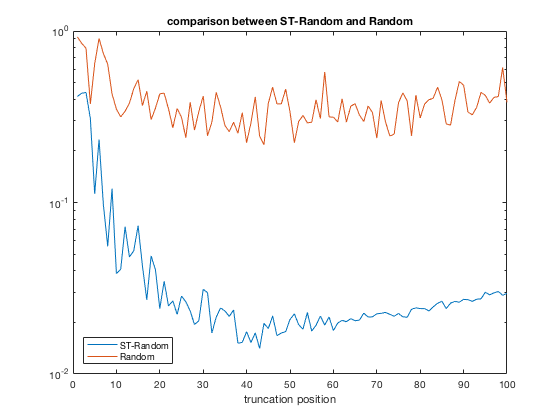
\includegraphics[scale=0.7]{tensorRandom}}

In the figure above, "ST" means "sequentially truncated". We use the relative difference between the error produced by our algorithm and the error by HOOI, which is usually considered in practice as the best approximation of a fixed core tensor size. Precisely, the y-axis of the figure represents:
$$ \frac{\epsilon_{algorithm} - \epsilon_{HOOI}}{\epsilon_{HOOI}}.$$

We mention that this criterion will be used in later experiments.

The tensor used in our experiments are $200 \times 200 \times 200$ random tensors. We see that the sequentially truncated version for this random algorithm greatly outperforms the one without sequential truncation. And the relative difference is about $1\%-2\%$.

As a property of the random tensor of uniform distribution, when it is regarded as a matrix, the biggest singular value is drastically bigger than the remaining. As a remedy, we can apply the enhancement techniques introduced in \cite{randAppro}. That is, for extracting samples, we use
$$ Y_i := (C_i C_i^T) C_i \Omega_i$$
to replace the original $Y_i :=  C_i \Omega_i$. Intuitively, this approach will enlarge the difference between big and small singular values, and reduce the probability of a wrong sample, which is fairly important in our case since the wrong choice of the leading vector will leads a large error.

This has been proved by experiment:

\centerline{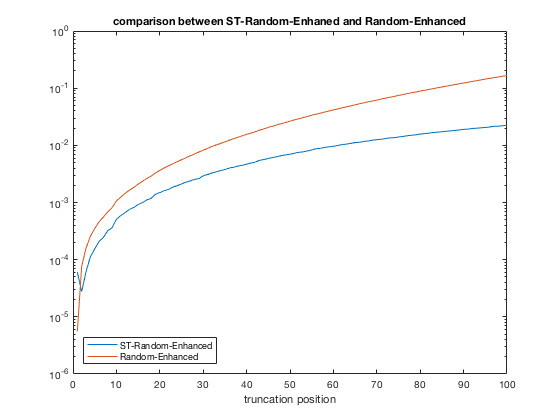
\includegraphics[scale=0.7]{tensorRandomEnh}}

In this figure, we use the enhanced version to approximate the same tensors. There is apparent improvement in terms of accuracy. Moreover, when the truncation position is small, the relative difference of error has even been shrinked to a $0.01\%$ level.



One of the most time-consuming part in this randomized algorithm is the computation of the tensor matrix multiplication, namely $Y_i := C_i \Omega_i$ in the statement of the algorithm. However, from the perspective of parallel computing, when the tensor is distributed in memory by the multidimensional layout, this tensor matrix multiplication can be easily parallelized, such that every processor nearly only needs to compute its local part of multiplication.

\subsection{QRCP Based Algorithm}

The original QR algorithm factorize a matrix $A$ into $A = QR$, where $Q$ is an orthogonal matrix, and $R$ is upper triangular. However, in this original version the computation of $Q$ and $R$ cannot be truncated at some intermediate point, because there is no reasonable error control if the decomposition is not complet. 

Fortunately, with a column pivoting, this disadvantage can be partially remedied. QR decomposition with column pivoting, or simply QRCP, is a modified QR decomposition where the final result of this decomposition is of the form
$$AP = QR,$$
where $P$ is a permutation matrix.

A well-known QRCP algorithm based on the Household reflection is as follows: at every stage of the loop, pivot the column of the maximal norm to the front, and the remaining steps are the same as the original QR algorithm. Since the column norms are examined in the procedure, we can know how much error will be incurred if we stop factorizing at a specific point. To be clarified, consider an intermediate snapshot during a whole decomposition:
$$
A P_c = Q
\begin{pmatrix}
R_{11} & R_{12}  \\
           & R_{22}
\end{pmatrix},
$$
Traditional QRCP algorithm chooses the column in $R_{22}$ with maximal norm, and then permutes it to the front. Thus if we stop at this point, the Frobenius error of this truncation will be bounded by 
$$ || R_{22} || ^2 = \sum_{i} || R_{22}(:,i) || ^2,$$

where $R_{22}(:,i)$ denotes the $i$th column of matrix $R_{22}$. Hence, if we employ this QRCP algorithm to each step of Tucker decomposition, an \textit{a posteriori} error estimate can be easily obtained from Theorem \ref{tuckerm1}. As a note of nomenclature, because this QRCP algorithm can be used to determine the rank of a matrix by truncating at a point where $||R_{22}||$ is sufficiently small, it is also called RRQR(Rank Revealing QR).

However, QRCP algorithm can do more if we pivot the columns with more refined strategies. In \cite{qrcp}, a strong rank reveal QR algorithm is proposed. 

\begin{mythm} ( see \cite{qrcp} )
\label{strongqrcpthm}
Let $A$ be an $m \times n$ matrix and let $ 1 \leq k \leq \min(m, n)$. For any given parameter $f > 1$, there exists a permutation $P_c$ and a QR decomposition
$$
A P_c = Q
\begin{pmatrix}
R_{11} & R_{12}  \\
           & R_{22}
\end{pmatrix},
$$
such that 
$$ 1 \leq \frac{\sigma_i(A)}{\sigma_i(R_{11})} , \frac{\sigma_j(R_{22})}{\sigma_{k+j}(A)} \leq \sqrt{ 1 + f^2 k (n - k)}$$
is satisfied for any $1 \leq i \leq k$ and $1 \leq j \leq \min(m, n) - k$.
\end{mythm}

An QR decomposition satisfying this theorem is called a strong RRQR. An efficient algorithm to compute the permutation for strong RRQR exists. Roughly speaking, it is based on continuously permuting 2 columns until a quantity is sufficiently small, the satisfaction of which implies that such permutation is already a strong RRQR. For detailed description, we refer to Algorithm 4 in \cite{qrcp}.

We can apply this rank revealing QR algorithm to approximate a tensor as follows:
\begin{myalgo}
Suppose we are given a tensor $\mathcal{A}$ of size $n_1 \times \dots \times n_d$ to decompose. 
\begin{itemize}
\item initialization: set $\mathcal{A}_0 \leftarrow \mathcal{A}$
\item for $i$ from $1$ to $d$: 
	\begin{itemize}
		\item compute $\mathcal{A}_{i-1} \approx \mathcal{A}_i \times_i Q_i $ by applying RRQR algorithm
	\end{itemize}
\item finalization: set $\mathcal{B} \leftarrow \mathcal{A}_d$, obtain $\mathcal{A} \approx  \mathcal{B} \times_1 Q_1 \dots \times_d Q_d $
\end{itemize}
\end{myalgo}

\begin{mythm}
Suppose in the algorithm above, we are using the strong RRQR algorithm, and let $\tilde{\mathcal{A}} :=  \mathcal{B} \times_1 U_1 \dots \times_d U_d $, $A_{best}$ be the best approximation with the same core tensor size, then the error produced by the algorithm above satisfies:
$$ || \mathcal{A} - \tilde{\mathcal{A}} || \leq \sqrt{1 + f^2 \Pi_{i = 1}^d n_d} || \mathcal{A} - \mathcal{A}_{best} || $$
\end{mythm}

\begin{proof}
First of all, we deduce more information from Theorem \ref{strongqrcpthm}. We keep all the notations of Theorem \ref{strongqrcpthm}:
\begin{alignat*}{9}
 || R_{22} || ^ 2 & = \sum_{j = 1}^{\min(m, n) - k} \sigma_j (R_{22})^2 \\
 & \leq (1 + f^2k(n-k)) \sum_{j = k + 1} ^ {\min(m, n)} \sigma_j (A) ^ 2 \\
 & \leq (1 + f^2k(n-k)) || A - A_{svd\_at\_k} || ^ 2 \\
 & \leq (1 + f^2mn) || A - A_{svd\_at\_k} || ^ 2 .
\end{alignat*}
where $\mathcal{A}_{svd\_at\_k}$ denotes the approximation produced by the truncated SVD at $k$. On the other hand, the truncation in the RRQR algorithm, precisely, is:
$$ 
\tilde{A}P_c := Q
\begin{pmatrix}
R_{11} & R_{12}  \\
           & 0
\end{pmatrix}.
$$
Thus the Frobenius error of the matrix truncation, can be bounded by:
$$ || A - \tilde{A} || = || R_{22} || \leq \sqrt{1 + f^2mn} || A - A_{svd\_at\_k} || .$$

This result is general, provided that the hypothesis of Theorem \ref{strongqrcpthm} holds. Applying to our particular case, $mn$ can always be bounded by $\Pi_{i = 1}^d n_d$. Thus, once we utilize the tactic used before, we obtain:
$$ || \mathcal{A} - \tilde{\mathcal{A}} || \leq \sqrt{1 + f^2 \Pi_{i = 1}^d n_d} || \mathcal{A} - \mathcal{A}_{best} || $$
\end{proof}

This theoretical is not so attractive, since the term $\Pi_{i = 1}^d n_d$ might normally be an extremely large number. However, according to our numerical experiments, the magnitude of error is far below this prediction.

\centerline{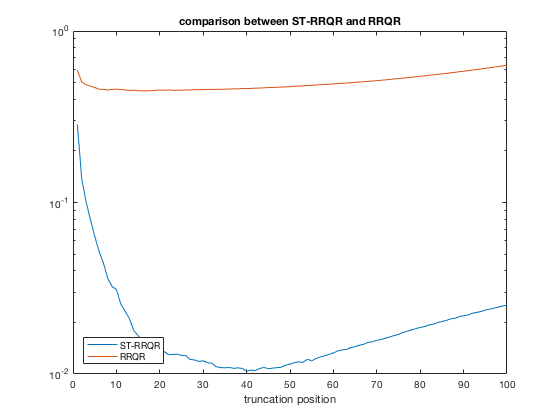
\includegraphics[scale=0.7]{tensorRRQR}}

The experiment is carried out for random tensors of size $200 \times 200 \times 200$. As in the case of the random algorithm above, we can define the similar version without sequential truncation. In the experiments, we see once more that sequentially truncated version is generally much better than the one without it. The practical error found in the figure is very similar to the randomized algorithm above as well.

We can use the same technique to improve the result as we have done in the randomized algorithm. That is, we use matrix
$$ (AA^T)A := QRP^T$$
to compute the QRCP.

The result is shown in the following figure:


\centerline{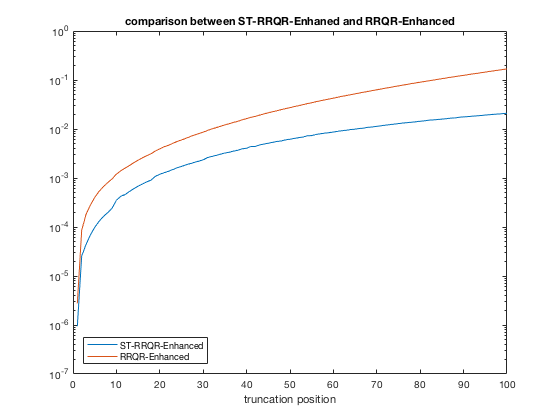
\includegraphics[scale=0.7]{tensorRRQREnh}}

According to the experiment, the final error is significantly improved, especially when the truncation position is small. Intuitively, it can be explained as a result of intensified difference in singular values, which ensures that the pertinent columns will be larger and more likely to be pivoted to the front. However, the author doesn't have a strict theoretical proof of this phenomenon.

On the other hand, if we use strong RRQR instead, we have a theoretical explanation: 

\begin{mythm}
\label{rrqrenh}
Let $A$ be an $m \times n$ matrix. Fix $q \geq 0$. We compute the strong RRQR of parameter $f > 1$ for 
$$ (AA^T) ^q  AP \approx QR, $$
with truncation at position $k$. Then $QQ^TA$ is also an approximation of $A$, satisfying
$$ || A - QQ^TA || \leq  (m-k)^\frac{2q}{2q+1} (1 + f^2k(n-k))^\frac{1}{2(2q+1)} || A - A_{svd\_at\_k} ||  $$
\end{mythm}

Instead of the proof, we first have a closer look at what this theorem implies. The factor $(1 + f^2k(n-k))$ is tremendously reduced to $(1 + f^2k(n-k))^\frac{1}{2q+1}$, at the expense of a new incurred factor bounded by $(m-k) ^ \frac{2q}{2q+1} \leq m - k$. In the case of tensor decomposition, especially for the initial steps, the matrix to be approximated is usually of size $m \times n$ with $m \ll n$. For such matrices, the theoretical bound of RRQR approximation will be significantly improved.

In order to prove this theorem, we the following lemma. We note once more that our matrix norm is always the Frobenius norm.
\begin{mylem}
Let $\pi$ be an orthogonal projection of size $m \times m$ onto a subspace of dimension $r$, $A$ be a matrix of size $m \times n$. For any integer $q \geq 0$,
$$ || \pi A || \leq  r^\frac{2q}{2q+1} || \pi (AA^T)^q A || ^ {1/(2q + 1)}.$$
\end{mylem}
\begin{proof}
We can always assume that $A$ is a diagonal matrix with nonnegative entries without loss of generality, because otherwise we can replace $A$ by $\Sigma$, where
$$ A = U\Sigma V^T $$
is the singular decomposition of $A$. Furthermore, a orthogonal projection is always of the form $\pi = PP^T$, where $P$ is a column full rank matrix of size $m \times r$ with orthonormal columns.

Thus the desired inequality is equivalent to
$$ || P^TA || \leq || P^T(AA^T)^q A ||, $$
where $A$ is diagonal. We denote its diagonal entries as $\sigma_i$'s. Then by the definition of Frobenius norm, the inequality is equivalent to 
$$ \sum_{i = 1}^r \sigma_i^2 \leq r^\frac{2q}{2q+1} (\sum_{i = 1}^r (\sigma_i ^ 2) ^ {2q+1}) ^ \frac{1}{2q+1}$$ 
It is obviously true, because we have the arithmetic mean inequality:
$$ \frac{\sum_{i = 1}^r \sigma_i^2}{r} \leq (\frac{\sum_{i = 1}^r (\sigma_i ^ 2) ^ {2q+1}}{r}) ^ \frac{1}{2q+1}.$$ 
\end{proof}

\begin{proof}{(Theorem \ref{rrqrenh})} 
By Theorem \ref{strongqrcpthm} for $(AA^T)^q A$, we have
\begin{alignat*}{9}
& || (AA^T)^q A - QQ^T (AA^T)^q A || \\
\leq &(1 + f^2k(n-k))^\frac{1}{2} \sum_{i = k+1}^{\min(m,n)} \sigma_i((AA^T)^q A) \\
= & (1 + f^2k(n-k))^\frac{1}{2} \sum_{i = k+1}^{\min(m,n)} \sigma_i(A) ^ {2q+1} \\
\leq & (1 + f^2k(n-k))^\frac{1}{2} || A - A_{svd\_at\_k} || ^ {2q+1}.
\end{alignat*}

On the other hand, since $I - QQ^T$ is an orthogonal projection onto a subspace of dimension $m - k$, by the lemma above, we obtain
$$|| A  - QQ^TA || \leq  (m-k)^\frac{2q}{2q+1} || (AA^T)^q A - QQ^T (AA^T)^q A || ^\frac{1}{2q+1}. $$
Therefore, the desired inequality is a combination of these two.

\end{proof}


With 1-dimensional memory layout, we remark that RRQR algorithm can be parallelized, allowing a reasonable error bound. We refer to \cite{carrqr} for details.


\subsection{Further Generalization}
We will explore more in this subsection on possible generalizations of Tucker decomposition. We define a Tucker decomposition before in Definition \ref{tuckerd} as an approximation
$$ \mathcal{A} \approx \mathcal{B} \times_1 U_1 \dots \times_d U_d, $$
where $U_i$, $1 \leq i \leq d$ are matrices with orthonormal columns. The necessity of the orthogonality of these factor matrice is based on 2 observations: 1), If the decomposition is carried out with the original tensor in every step, then the orthogonality of $U_i$'s provides an easy way to construct the final core tensor $\mathcal{B}$, since $U^TU$ is actually a smaller identity matrix. 2), Theorem \ref{tuckerm1} is a precise formula to compute the accumulated error by all steps, which is a consequence of the fact that $UU^T$ is an orthogonal projection.

However, if we choose to use a sequentially truncated scheme exclusively, then the decomposition can be constructed simultaneously during the process, without any extra computation of the core tensor, circumventing the first restriction. In the mean time, if we scale the resulting matrices a little and impose a bound to its biggest singular value, a practical error estimate can be calculated as in Theorem \ref{tuckerm1}, replacing the equality by an inequality. Thus the second restriction is not an insuperable obstacle. We can introduce a generalized version of Tucker decomposition as follows:

\begin{mydef}{(Generalization of Tucker Decomposition)}
Let $\mathcal{A}$ be a tensor of size $n_1 \times \dots \times n_d$. A generalized Tucker decomposition of $\mathcal{A}$ is comprised of 1), a core tensor $\mathcal{B}$ of size $m_1 \times \dots \times m_d$; 2) a collection of matrices $M_i$, $1 \leq i \leq d$ of size $n_i \times m_i$ respectively, satisfying $\sigma_1(M_i) \leq 1$, $\forall 1 \leq i \leq d$. The core tensor together with the collection of matrices should give an approximation of the original tensor by
$$ \mathcal{A} \approx \mathcal{B} \times_1 M_1 \dots \times_d M_d $$
\end{mydef}

In fact, this generalized Tucker decomposition sets up a mapping from all algorithms factorizing a matrix $A$ to $A \approx M B$ with $\sigma_1(M_i) \leq 1$, to a tensor decomposition of format $ \mathcal{A} \approx \mathcal{B} \times_1 M_1 \dots \times_d M_d $. As will be illustrated later, the error of this tensor decomposition can be estimated by the error of matrix truncation in each step.

\begin{myalgo}
Suppose we have a matrix decomposition algorithm, decomposing $A$ to $A \approx M B$ with $\sigma_1(M_i) \leq 1$. We can construct an algorithm to produce a tensor decomposition algorithm as follows:
\begin{itemize}
\item initialization: set $\mathcal{A}_0 \leftarrow \mathcal{A}$
\item for $i$ from $1$ to $d$: 
	\begin{itemize}
		\item compute $\mathcal{A}_{i-1} \approx \mathcal{A}_i \times_i M_i $ by the given matrix algorithm
	\end{itemize}
\item finalization: set $\mathcal{B} \leftarrow \mathcal{A}_d$, obtain $\mathcal{A} \approx  \mathcal{B} \times_1 M_1 \dots \times_d M_d $
\end{itemize}
\end{myalgo}

\begin{mythm}
In the tensor decomposition algorithm above, suppose that at step $i$ of the "for" loop, we get a truncation error
$$ || \mathcal{A}_{i-1} - \mathcal{A}_i \times_i M_i || \leq \epsilon_i. $$
Then the final approximation error is controlled by 
$$ || \mathcal{A} - \mathcal{B} \times_1 \dots \times_d M_d || \leq \sum_{i = 1}^d \epsilon_i. $$
\end{mythm}

\begin{proof}
We prove the following inequality by mathematical induction:
$$ || \mathcal{A} - \mathcal{A}_s \times_1 \dots \times_s M_s || \leq \sum_{i = 1}^s \epsilon_i , \forall 1 \leq s \leq d $$
The original inequality is the special case when $s$ is set to $d$.

When $s = 1$, the inequality holds trivially.

Suppose the inequality holds for $s$($1 \leq s \leq d - 1$), we will prove it is still valid for $s + 1$:
Since $M_i$, $1 \leq i \leq d$ satisfies $\sigma_1(M_i) \leq 1$, $M_i$ will decrease the $l_2$ norm of a vector when applying to it. Thus for any tensor $\mathcal{C}$ of compatible size, we have
$$|| \mathcal{C} \times_i M_i || \leq || \mathcal{C} ||, $$
We multiply $M_1, \dots M_s$ successively to the left of the inequality:
$$ || \mathcal{A}_s - \mathcal{A}_{s+1} \times_{s+1} M_{s+1} || \leq \epsilon_{s+1}, $$
leading
$$ || \mathcal{A}_s \times_1 \dots \times_s M_s - \mathcal{A}_{s+1} \times_1 \dots \times_s M_s \times_{s+1} M_{s+1} || \leq \epsilon_{s+1}. $$
As a consequence,
\begin{alignat*}{9}
 &|| \mathcal{A} - \mathcal{A}_{s+1} \times_1 \dots \times_{s+1} M_{s+1} || \\
 \leq & || \mathcal{A} - \mathcal{A}_s \times_1 \dots \times_s M_s || + || \mathcal{A}_s \times_1 \dots \times_s M_s - \mathcal{A}_{s+1} \times_1 \dots \times_{s+1} M_{s+1} || \\
 \leq & || \mathcal{A} - \mathcal{A}_s \times_1 \dots \times_s M_s || + \epsilon_{s+1} \\
 \leq & \sum_{i = 1}^{s+1} \epsilon_i
\end{alignat*}
\end{proof}

\begin{myrmk}
The theorem above still holds for the HOSVD algorithm with sequential truncation. However, the result is weakened to an inequality because we only take advantage of the upper bound of the biggest singular value and ignore the orthogonality of the matrices.
\end{myrmk}

\begin{comment}
This new generalization of Tucker decomposition removes the necessity of any orthogonality, thus opens the door for any matrix approximation algorithms to be applied in the Tucker decomposition, allowing well-behaved final approximation error accumulated by the error incurred in each step. For instance, we refer to \cite{lucrtp}, where a rank revealing LU decomposition algorithm is presented in the parallel computing setting. This truncated LU decomposition with both row and column pivoting, called LU\_CRTP, can approximate a matrix with theoretical error bound. An algorithm like this has potential applicability in this generalized Tucker decomposition. 
\end{comment}

\section{Tensor Train Decomposition}
Although Tucker decomposition is an effective way to reduce the data size for 3 or 4 dimensional problem, the space needed to store expands exponentially as the dimension grows. For example, consider a tensor of dimension $d$ with the length in every dimension $n$. For storing the original tensor, we need $n^d$ space. If we truncate this tensor with Tucker decomposition at threshold $k$ uniformly, we still need $k^d + knd$ space. Since the dimension $d$ appears as an exponent in the final representation, the storage becomes inacceptable soon as $d$ grows.

The scenario where $d$ is significantly high is not rare in these day's applications, including computational finance, quantum chemistry, and stochastic partial differential equations. When $d$ becomes as high as 100 or even 1000, we must find out a new representation scheme to break the curse of dimensionality.


\begin{mydef}{(Tensor Train Decomposition)}
Let $\mathcal{A}$ be a tensor of size $n_1 \times \dots \times n_d$. A tensor train decomposition of $\mathcal{A}$ consists of a collection of 3-dimensional tensors:
$$ G_1, G_2, \dots, G_d,$$
where $G_i$ is of size $n_i \times r_{i-1} \times r_i, \forall 1 \leq i \leq d$, with $r_0 = r_d = 1$.

This collection of 3-dimensional tensors defines an approximate $\tilde{\mathcal{A}} \approx \mathcal{A}$ by:
$$ \tilde{\mathcal{A}} (i_1, \dots, i_d) :=  \sum_{1 \leq t_0 \leq r_0, \dots 1 \leq t_d \leq r_d} G_1(i_1, t_0, t_1) \dots G_d(i_d, t_{d-1}, t_d).$$
\end{mydef}


This definition has a relatively intuitive explanation. We fix $1 \leq s \leq d$ and $1 \leq i_s \leq n_s$. Then $G(i_s) := G(i_s, \cdot, \cdot)$ can be naturally regarded as a matrix.
And the approximate above is actually:
$$ \mathcal{A}(i_1, \dots, i_d) \approx G_1(i_1)G_2(i_2) \dots G_d(i_d),$$

On the other hand, constants $r_0, r_1, \dots, r_d$ indicate the degree of truncation, which play the same role as the core tensor size in Tucker decomposition. When these constants are fixed, the TT-decomposition possesses a best approximation.

\begin{myprop}
Let $\mathcal{A}$ be a tensor of size $n_1 \times \dots \times n_d$. Let $r_0, r_1, \dots, r_d$ be fixed positive integers with $r_0 = r_d = 1$. Then there exist a collection of 3-dimensional tensors $\{G_i\}_{i = 1}^d$, where $G_i$ has size $n_i \times r_{i-1} \times r_i$, such that for any other collection $\{G_i'\}_{i=1}^d$ with the same size, $\{G_i\}_{i=1}^d$ would not produce worse approximation than $\{G_i'\}_{i=1}^d$.
\end{myprop}

\begin{proof}
Similar to the counterpart of this proposition of the Tucker decomposition.
\end{proof}

However, one of the major difficulties for illustrating an algorithm of this decomposition scheme is about notation. Because tensor train decomposition is mainly for high dimensional tensor, there are more interaction between different dimensional indices. In Tucker decomposition, we regard a tensor as a juxtaposition of vectors step by step, which is the only interaction between different modes. However, in TT-decomposition, we need to re-interpret a tensor as a matrix in multiple ways. Thus we first introduce the following definition of general metricization. Conceptually, it is simply. Because any tensor of size $n_1 \times \dots \times n_d$ can be grouped into $ (n_1 n_2 \dots n_s) \times (n_{s+1} \dots n_d)$, which naturally defines a way of interpreting it as a matrix. The following definitions articulate this intuitive concept.


\begin{mydef}{(Alphabetical Mapping)}
Let $n_1, \dots, n_d$ be $d$ positive integers. Let $A := \{( i_1, \dots, i_d ) : 1 \leq i_s \leq n_s, \forall 1 \leq s \leq d \}$ be a set of tuples, and $B := \{1, \dots, \Pi_{s=1}^dn_s\}$ be a set of integers. Then the bijection  $\phi : A \rightarrow B$ determined by the alphabetical order of elements in $A$ is called the alphabetical map from $A$ to $B$.
\end{mydef}

\begin{mydef}{(General Metricization)}
Let $\mathcal{A}$ be a tensor of size $n_1 \times \dots \times n_d$. Let $s$ be a constant satisfying $1 \leq s \leq d$, and $S_1 := (p_1, \dots, p_s), S_2 := (p_{s+1}, \dots, p_d)$
be a disjoint partition of $\{1, \dots, d\}$. Denote $l_1 := \Pi_{i = 1}^s p_i, l_2 := \Pi_{i = s+1}^d p_i$. Then denote $\phi_1$ to be the alphabetical mapping from 
$$\{(i_{p_1}, \dots, i_{p_s}): 1 \leq i_{p_1} \leq n_{p_1}, \dots, 1 \leq i_{p_s} \leq n_{p_s} \}$$
to $\{1, \dots, l_1\}$. Similarly we can define $\phi_2$.

Then a general matricization of $\mathcal{A}$ with respect to the partition $(S_1, S_2)$ is the matrix defined element-wise by:
$$ M(u, v) := \mathcal{A}' ( \phi_1^{-1}(u), \phi_2^{-1}(v) ), $$
where $\mathcal{A}'$ is defined by:
$$ \mathcal{A}'( (i_{p_1}, \dots, i_{p_s}), (i_{p_{s+1}}, \dots, i_{p_d})) := \mathcal{A}(i_1, \dots, i_d)$$
\end{mydef}

The definition of general matricization is a little lengthy, however, it facilitates and clarifies the explanation of regarding a tensor as a matrix in a general manner. And a trivial but important observation about general matricization is the consistency of Frobenius norm, which is also one of the major reason that the Frobenius norm is the \textit{de facto} standard norm to analyze tensor approximations.

\begin{myprop}
Let $\mathcal{A}$ be a tensor. Suppose $A$ is any general matricization of $\mathcal{A}$, then
$$ || \mathcal{A} || = || A ||, $$
where the norms in left and right side are tensor Frobenius norm and matrix Frobenius norm respectively.
\end{myprop}
\begin{proof}
The square of both sides is the square sum of all the entries.
\end{proof}

\subsection{Computing TT-decomposition}
As is similar to the Tucker decomposition, we will present the TT-decomposition algorithm in a general setting. In fact, as long as we have a matrix decomposition algorithm providing
$ A \approx QB $, 
where $Q$ has orthonormal columns and $B$ is computed from $B = Q^TA$, we can construct an TT-decomposition algorithm. And this constructed algorithm allows an error estimation based on the truncation error incurred in each step.

\begin{myalgo}
Let $\mathcal{A}$ be a tensor of size $n_1 \times \dots \times n_d$, and we are given a matrix approximation algorithm decomposing a matrix into an orthonormal matrix and an arbitrary matrix. Then we can construct a TT-decomposition of tensor $\mathcal{A}$ as follows:
\begin{itemize}
\item initialization: set $\mathcal{A}_0 \leftarrow \mathcal{A}$, regard it as a tensor of size $r_0 \times n_1 \times n_2 \times \dots \times n_d$ (since $r_0 = 1$, it's always possible)
\item for $i$ from $1$ to $d$:
	\begin{itemize}
		\item $\mathcal{A}_{i-1}$ is a tensor of size $r_{i-1} \times n_i \times \dots \times n_d$, general-matricize it at $((r_{i-1}, n_i), (n_{i+1}, \dots, n_d))$ to a matrix $A_{i-1}$. Perform the given matrix decomposition algorithm on $A_{i-1} \approx Q_iB_i$ with truncation at rank $r_i$. Thus $Q_i$ can be regarded as a general matricization of a tensor $G_i$ of size $n_i \times r_{i-1} \times r_i$, and $B_i$ can be regarded as a general matricization of a tensor $\mathcal{A}_i$ of size $r_i \times n_{i+1} \times \dots \times n_d$. \\
		Store $G_i$ as one of our desired output, use $A_i$ in the next turn of loop.
	\end{itemize}
\item finalization: output $G_1, \dots, G_d$
\end{itemize}
\end{myalgo}

The following theorem allows us to bound the final approximation error by the truncation error introduced in each step:

\begin{mythm}
\label{tterror}
We keep the hypothesis in the algorithm above. Let $\tilde{\mathcal{A}}$ be defined by 
$$ \tilde{\mathcal{A}} (i_1, \dots, i_d) :=  \sum_{1 \leq t_0 \leq r_0, \dots 1 \leq t_d \leq r_d} G_1(i_1, t_0, t_1) \dots G_d(i_d, t_{d-1}, t_d).$$
Then the approximation error can be calculated by:
$$ || \mathcal{A} - \tilde{\mathcal{A}} || ^ 2 = \sum_{i=1}^d || A_{i-1} - Q_iB_i || ^ 2. $$
\end{mythm}

\begin{proof}
The proof is based on a simple observation: 

If $A_{k-1} \approx Q_kQ_k^TA_{k-1} = Q_kB_k$, and $B_k$ is further approximated by $B_k \approx C$, then because $Q_kQ_k^T$ is an orthogonal projection,
\begin{alignat*}{9}
 & ||A_{k-1} - Q_kC|| ^ 2 \\
= & || (I - Q_kQ_k^T)A_{k-1} + Q_k(B_k - C) || ^ 2  \\
=  & || (I - Q_kQ_k^T)A_{k-1} || ^ 2 + || Q_k(B_k - C) || ^ 2 \\
= & || A_{k-1} - Q_kB_k || ^ 2 + || B_k  - C || ^ 2
\end{alignat*}
Notice that this holds for whatever $C$, as long as $C$ is compatible with $B$ in terms of size. Therefore, by applying this equality recursively, we obtain the original equality.
\end{proof}

\begin{myrmk}
We note here that the restriction of the orthogonality of $Q_i$ is not essentially necessary. As in the case of generalized Tucker decomposition, this restriction can be weakened by $\sigma_1(M_i) \leq 1$(we use $M_i$ to denote $Q_i$, as an emphasis of the drop of orthogonality). As a result, the error estimate would become:
$$ || \mathcal{A} - \tilde{\mathcal{A}} || \leq \sum_{i=1}^d || A_{i-1} - M_iB_i ||,$$
whose proof is based on
\begin{alignat*}{9}
 & ||A_{k-1} - M_kC|| \\ 
=  & || A_{k-1} - M_kB_k || + || M_k(B_k - C) || \\
\leq & || A_{k-1} - M_kB_k || + || B_k  - C ||.
\end{alignat*}
However, with the consideration of a potentially big $d$, as is the design purpose of TT-format, this estimate of final error might be rough.
\end{myrmk}

\begin{myrmk}
An interesting implication of this theorem is that TT-format can be an exact decomposition, i.e. $\mathcal{A} = \tilde{\mathcal{A}}$, at the expense of potentially enormous $r_i$'s. In fact, we only need to use the exact SVD decomposition in every step, then this theorem guarantees that the final error is also 0. And we can get a better understanding of why TT-format is particularly suitable for high dimension tensors. If a reasonable error can be achieved by truncating at small $r_i$'s, then the total memory used to store the TT-format is only:
$$ \sum_{i = 1}^d n_i  r_{i-1} r_i. $$
Note that the dimension $d$ is no longer an exponent, thus the exponential growth of storage with respect to $d$ is avoided.
\end{myrmk}

The algorithm above is abstract, in the sense that the matrix decomposition algorithm can be any one based on an orthogonal projection. The most common choice of this kind of algorithm is truncated SVD. Since we have proved the existence of best approximation for TT-decomposition, if we use truncated SVD to approximate $A_{i-1}$, one might expect a similar relation between the final result of this algorithm and  the best approximation as in the Tucker decomposition. Fortunately, this is the case:

\begin{mythm}
We fix the constants $r_0, \dots, r_d$. If in the algorithm above, we use the truncated SVD as a specific matrix approximation algorithm, then the result $\tilde{\mathcal{A}}$ computed from this algorithm satisfies:
$$ || \tilde{\mathcal{A}} - \mathcal{A} || \leq \sqrt{d} || \mathcal{A}_{best} - \mathcal{A} ||,$$
where $\mathcal{A}_{best}$ is the best approximation of $\mathcal{A}$ with respect to the given $r_0, \dots, r_d$.
\end{mythm}

\begin{proof}
We use all notations in the statement of this algorithm. Let $\mathcal{A}_{best, i}$ be the tensor of size $r_i \times n_{i+1} \times \dots \times n_d$, obtained by multiplying $Q_1^T, \dots, Q_i^T$ successively for the same sequence of general matricization as we compute $\mathcal{A}_i$. Since $Q_i^T$ is a projection to a smaller space, we have:
$$ || \mathcal{A} - \mathcal{A}_{best} || \geq || \mathcal{A}_i - \mathcal{A}_{best, i} || \geq || A_i - Q_{i+1}B_{i+1} ||. $$
Thus 
$$ || \mathcal{A} - \tilde{\mathcal{A}} || ^ 2 = \sum_{i=1}^d || A_{i-1} - Q_iB_i || ^ 2 \leq d || \mathcal{A}_{best} - \mathcal{A} || ^ 2. $$
\end{proof}

\subsection{Tensor Tree Decomposition}
Tensor tree decomposition is a generalization of the tensor train format. First, we need to have a closer look on the TT-format algorithm. The essential pattern in this algorithm can be summarized to a successive application of general matricization and matrix decomposition:
\begin{alignat*}{9}
& r_{i-1} \times n_i \times \dots \times n_d \\
\Rightarrow & (r_{i-1}n_i) \times (n_{i+1} \dots n_d) \\
\Rightarrow & (r_{i-1}n_i) \times r_i \text{ and } r_i \times  (n_{i+1} \dots n_d) \\
\Rightarrow & r_{i-1} \times n_i \times r_i \text{ and } r_i \times n_{i+1} \times \dots \times n_d
\end{alignat*}

This TT-format thus fixes the pattern of dimensional indices, where the generalization to tensor tree format takes place. In fact, tensor tree decomposition seeks more flexibility in this matricization and decomposition pattern. Instead of using a fixed sequential pattern, successively leaving the factor $r_{i-1} \times n_i \times r_i$ untouched afterwards, the tensor tree format employs a binary tree structure, and perform decomposition on both sides.

We use the first step for explanation. The general matricization is no longer restricted on the first 1 or 2 indices, instead, it can be at any point $1 < s_1 < d$ (or even with a permutation of all indices first, which is not shown bellow):
\begin{alignat*}{9}
&n_1 \times \dots \times n_d \\
\Rightarrow &  (n_1 \dots n_{s_1}) \times (n_{s_1+1} \dots n_d) \\
\Rightarrow & (n_1 \dots n_{s_1}) \times r_1 \text{ and } r_1 \times (n_{s_1+1} \dots n_d) \\
\Rightarrow & n_1 \times  \dots \times n_{s_1} \times r_1 \text{ and } n_{s_1+1} \times \dots \times n_d \times r_1
\end{alignat*}

Thus after the first step, we obtain 2 tensors with size $n_1 \times  \dots \times n_{s_1} \times r_1$ and $ n_{s_1+1} \times \dots \times n_d \times r_1$ respectively. And we can continue this procedure for both, and recursively form a binary tree structure.

There are several points worth mentioning for the tensor tree structure:

1) By suitably allocating the additional indices, i.e. $r_i$'s, it is always possible that at every level of the binary tree, there are exactly 2 tensors having 1 additional $r$ index, and all of the others has exactly 2 such additional $r$'s. Because generally, the addtional $r$'s can be allocated as follows:
\begin{alignat*}{9}
& n_{p_1} \times \dots \times n_{p_2} \times r_1 \\
\Rightarrow & n_{p_1} \times \dots \times n_{p_3} \times r_1 \times r_3 \text{ and } n_{p_3+1} \times \dots \times n_{p_2} \times r_2
\end{alignat*}
and
\begin{alignat*}{9}
& n_{p_1} \times \dots \times n_{p_2} \times r_1 \times r_2\\
\Rightarrow & n_{p_1} \times \dots \times n_{p_3} \times r_1 \times r_3 \text{ and } n_{p_3+1} \times \dots \times n_{p_2} \times r_2 \times r_3
\end{alignat*}
As a result, the final approximation formula of tensor tree format can be chosen to have the same form as the tensor train format.

2) After every decomposition, 2 resulting tensors become completely irrelevant to each other. Thus the following steps for these 2 tensors can be executed in an embarrassingly parallel manner. This parallelization might make this format potentially useful. 

3) None of the previously stated error estimation theorems for tensor train format still works. We recall the proof of those theorems for tensor train format, the crucial point is when we approximate $A$ by $A \approx MB$, $M$ will not be processed after that step, which ensures the error produced by further approximating $B$ won't be magnified too much, provided the norm of $M$ is small. However, in the tensor tree decomposition, this is not the case, since when an approximation is completed as $A \approx MB$, both $M$ and $B$ will be further approximated. Thus there is no way to impose restrictions on both $M$ and $B$ for a given general matrix $A$.

However, despite the lack of a fine estimation of error based on the error at each step, we can still deduct a weaker version for this kind of error estimation. For the clearance of statement, we use the truncated SVD in every step of decomposition:
$$ A \approx U \Sigma V^T.$$
Nevertheless, we will use a slightly different form to emphasize the symmetry of 2 resulting small tensors. The singular values $\Sigma$ will be stored separately, and 2 smaller tensor to be further processed are $U$ and $V$ (meaning their general matricization are $U$ and $V$). The following proposition estimates the final error at this node, with the final error at 2 children nodes already estimated:

\begin{myprop}
Let $|| A - U \Sigma V^T|| \leq \epsilon_0$, $|| U - \hat{U} || \leq \epsilon_1$ and $|| V - \hat{V} || \leq \epsilon_2$, then
$$ || A - \hat{U} \Sigma \hat{V}^T || \leq \epsilon_0 + (\epsilon_2 + \epsilon_1 + \epsilon_1 \epsilon_2) \sigma_1,$$
where $\sigma_1$ is the biggest singular value of $A$.
\end{myprop}

\begin{proof}
\begin{alignat*}{9}
& || A - \hat{U} \Sigma \hat{V}^T ||  \\
= & || (A - U \Sigma V^T) + U \Sigma (V^T - \hat{V}^T) + (U - \hat{U}) \Sigma \hat{V}^T ||  \\
\leq & \epsilon_0 + \epsilon_2 \sigma_1 + ||(U - \hat{U}) \Sigma (\hat{V}^T - V^T) + (U - \hat{U}) \Sigma V^T|| \\
\leq &  \epsilon_0 + \epsilon_2 \sigma_1 + \epsilon_1 \sigma_1 + \epsilon_1 \epsilon_2 \sigma_1
\end{alignat*}
\end{proof}

Thus we can estimate the final error of the tensor tree decomposition from leaves to root with the help of this inequality.


\begin{comment}
%latent variable models ==> natural language processing
\cite{tensorapplearn1}

%data mining, network analysis
\cite{tensorappmining1}
\cite{cpnetmining}

%recommandation system
\cite{tensorapprecom}

%computer vision 
\cite{tensorappvision}

%natural language processing
\cite{tensorapplang}

\cite{cpnpcomplete}
\cite{cpill} 

\cite{randAppro}
\cite{trand2007}
\cite{trandMACH}

\cite{lowranklit}
\cite{koldapara}

\cite{trunctucker}
\cite{Tucker1966}
\cite{tucker2000}

\cite{ttrain}
\cite{koldaapp}
\cite{ttree}

\cite{thiera}

\cite{qrcp}
\cite{carrqr}
\cite{lucrtp}

\cite{cpgigatensor}

\end{comment}


%\bibliographystyle{unsrt}
\bibliographystyle{apa}
\bibliography{mybib} 


\end{document}
